
\documentclass{letter}

\usepackage{csquotes}
\usepackage[margin=1in]{geometry}
\usepackage{tikz}
\usepackage{amsmath}
\usepackage{enumitem}

\newcommand{\heading}[1]{{\large \textsc{#1}}}

\begin{document}

\heading{COMP 282 - Quiz 3 (Spring, 2019)}
\kern 2cm
\heading{Name:}

{\bf Question 1} \kern 1cm Insert the value \texttt{6} into the following {\em
Red-Black Tree}.  Denote red nodes with a dashed outline, black nodes with a
solid circle, and double-black nodes with a double-solid circle.  Show {\em
ALL} steps.

\begin{center}
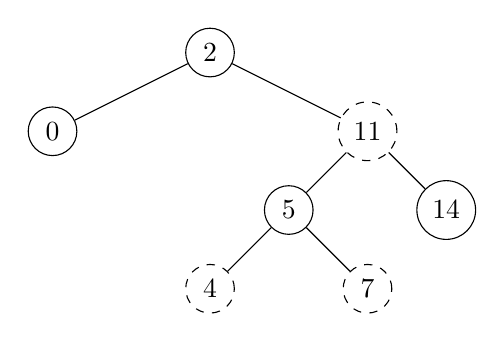
\begin{tikzpicture}
\node[shape=circle,draw=black] (2) at (0,0) {2};
\node[shape=circle,draw=black] (0) at (-2,-1) {0};
\node[shape=circle,draw=black,dashed] (11) at (2,-1) {11};
\node[shape=circle,draw=black] (5) at (1,-2) {5};
\node[shape=circle,draw=black,dashed] (4) at (0,-3) {4};
\node[shape=circle,draw=black,dashed] (7) at (2,-3) {7};
\node[shape=circle,draw=black] (14) at (3,-2) {14};

\path (2) edge (0);
\path (2) edge (11);
\path (11) edge (5);
\path (11) edge (14);
\path (5) edge (4);
\path (5) edge (7);
\end{tikzpicture}
\end{center}

\end{document}
